\begin{figure*}[t]
\centering
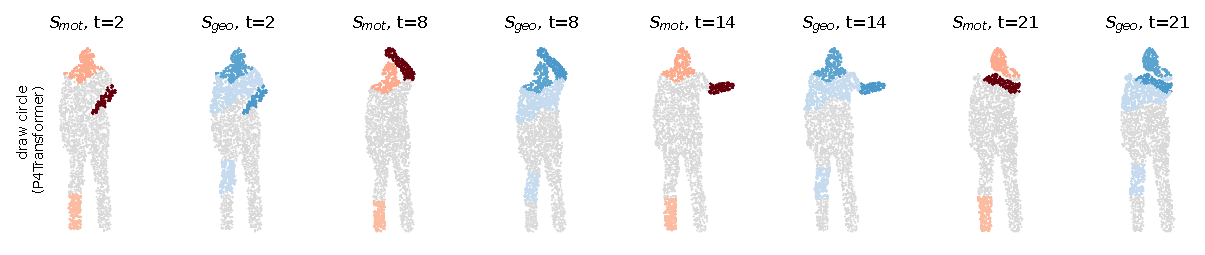
\includegraphics[width=\textwidth]{fig/msr_teaser.pdf}
\caption{\textbf{\methodlong\ (\method)} attributes a 4D model's decision to \emph{how} each spacetime region moves ($\Smot$, red) and to \emph{what shape} it has ($\Sgeo$, blue). It intervenes on the input and reads only the model's output. The clip is a real MSR-Action3D test clip (\emph{draw circle}) at four instants, explained for the official P4Transformer. The motion term is strongest on the drawing hand (weaker on the head and one foot), while geometry importance covers the upper body. Fig.~\ref{fig:qual} in the appendix shows two more actions on all three backbones, including one where the motion term falls on the torso. No attention, gradient or point correspondence is used, and the same code explains convolutional and attention-free state-space backbones (Sec.~\ref{sec:exp-cross}).}
\label{fig:teaser}
\end{figure*}

\section{Introduction}
\label{sec:intro}

Point-cloud video is the stream of 3D point sets produced by depth and LiDAR sensors, and it underpins action recognition, robotic manipulation, assistive monitoring and augmented reality. Dedicated \emph{4D} backbones now model it directly: point spatio-temporal convolutions~\cite{fan2021pstnet}, spatio-temporal transformers~\cite{fan2021p4transformer} and attention-free state-space models such as Mamba4D~\cite{liu2025mamba4d}. They are accurate but opaque. Before such a model is deployed, a practitioner should be able to check \emph{what} it bases a decision on. Did it label a clip ``high arm wave'' because of \emph{how} the arm moved, or because of \emph{what shape} the body had? A model that relies on shape where the task is defined by motion has learned a shortcut, as RGB action models do with static appearance~\cite{li2023staticbias}, and that shortcut can fail under new subjects, clothing or sensor placement.

\paragraph{What a deployable 4D explanation needs.}
We argue that an explanation method for deployed 4D models has to meet four requirements, and that no existing method meets them all.
\emph{(R1) Black-box access.} Deployed models are often compiled, quantised or served behind an interface, and the backbones differ in kind. Gradients need white-box access. Attention is a contested proxy for importance~\cite{jain2019attention,abnar2020rollout}, and Mamba4D has no attention to read. An explanation should therefore need only forward queries.
\emph{(R2) Real sensor data.} Sensors re-sample the surface in every frame, so ``the same point at two times'' does not exist. Any operator that moves or freezes indexed points silently breaks on real data.
\emph{(R3) The right question.} A prediction can depend on the \emph{shape} of a structure or on its \emph{motion}. In pixel space the two are entangled in one saliency value. In 4D they are physically distinct, yet 3D attribution is single-frame~\cite{zheng2019pointcloudsaliency,schinagl2022occam}, video attribution works on RGB pixels~\cite{price2020playfair,lee2025dance}, and no method attributes a decision to motion versus geometry.
\emph{(R4) Verifiable and affordable.} An explanation that will be acted on must be shown to be faithful to the model, must depend on the learned weights~\cite{adebayo2018sanity}, should be checked against ground truth where it exists, and must run at a practical cost.

\paragraph{Our approach.}
\methodlong (\method) treats explanation as intervention on tracked spacetime regions. Its key operator, \frz, holds a region static in its anchor-frame configuration: the region loses its motion and keeps its shape. A shape-free proxy that follows the region's centroid does the converse. The four resulting inputs form a motion$\times$geometry cube for each region. Averaging the cube's two paths yields an order-symmetric geometry term $\Sgeo$ and motion term $\Smot$ that sum exactly to the region's necessity $\Nec$, and the cube's mixed difference measures their interaction. All operators rewrite only a region's per-frame point \emph{sets}, so they need no correspondences. A context-averaged estimator, a Banzhaf-type average over random interventions on the other regions, keeps the scores reliable when a structure spans several regions. \method only queries the model, so it explains convolutional, attention and state-space backbones with the same code (Fig.~\ref{fig:teaser}).

\paragraph{Contributions.}
\begin{itemize}[leftmargin=1.2em,itemsep=2pt,topsep=2pt]
\item \textbf{\method, a black-box explanation that separates motion from geometry} (R1, R3). To our knowledge it is the first method that attributes a 4D model's decision to the \emph{motion} versus the \emph{geometry} of each spacetime region. Its decomposition is complete and order-symmetric (Shapley), and it reports the interaction instead of assuming it away (Sec.~\ref{sec:method}).
\item \textbf{A correspondence-free instantiation with guarantees} (R2). Set-based operators, a local and a context-averaged estimator, and the conditions under which each score is a causal effect.
\item \textbf{A validation protocol for deployment} (R4). On three unmodified official backbones we test faithfulness against 13 baselines, localisation against skeleton ground truth, dependence on the learned weights, stability under sensor re-sampling, and cost. We also give a \emph{crossover audit}: two tasks built from real clips whose classes differ only in the motion or only in the shape of one arm, which checks whether the explanation reports the cue a model was trained to use. The crossover is our primary evidence that the split is correct; the other tests show that it costs no faithfulness (Sec.~\ref{sec:exp}).
\end{itemize}
